\documentclass[10pt,conference]{IEEEtran}

% ---- Packages ----
\usepackage[utf8]{inputenc}
\usepackage{graphicx}
\usepackage{booktabs}
\usepackage{array}
\usepackage{hyperref}
\usepackage{xcolor}
\usepackage{tikz}
\usepackage{listings}
\usepackage{enumitem}
\usepackage{caption}
\usepackage{cite}
\usepackage{microtype}
\usetikzlibrary{shapes,arrows.meta,positioning}

% ---- Spacing ----
\setlength{\textfloatsep}{5pt plus 2pt minus 2pt}
\setlength{\floatsep}{5pt plus 2pt minus 2pt}
\setlength{\intextsep}{5pt plus 2pt minus 2pt}
\setlength{\columnsep}{16pt}
\setlist{nosep, leftmargin=12pt, topsep=2pt}
\captionsetup{font=small, skip=2pt}

% ---- Colors ----
\definecolor{isroblue}{RGB}{0, 51, 102}
\definecolor{codegreen}{RGB}{0,120,0}
\definecolor{codegray}{RGB}{100,100,100}
\hypersetup{colorlinks=true, linkcolor=isroblue, urlcolor=isroblue}

% ---- Code style ----
\lstset{
    basicstyle=\ttfamily\scriptsize,
    keywordstyle=\color{isroblue}\bfseries,
    commentstyle=\color{codegray},
    stringstyle=\color{codegreen},
    breaklines=true,
    breakatwhitespace=false,
    columns=fullflexible,
    keepspaces=true,
    frame=single,
    framesep=2pt,
    xleftmargin=1pt,
    xrightmargin=1pt,
    aboveskip=0pt,
    belowskip=0pt
}

% ---- Title ----
\title{Deliverable 2: Tool Integration, Agentic\\Traceability and Task Completion}

\author{
    \IEEEauthorblockN{Yashvardhan (Team Lead) \quad \textbullet \quad Team Member 2}
    \IEEEauthorblockA{
        \textit{Capstone Project 2025--2026}\\
        ISRO Chandrayaan-5 --- Generative Agents at Aryabhata Station\\
        \textit{Submitted: February 28, 2026}
    }
}

\begin{document}

\maketitle

% ---- Abstract ----
\begin{abstract}
This report presents Deliverable~2 of the ISRO Chandrayaan-5 capstone project, which simulates eight AI-powered \textit{Gagannauts} at Aryabhata Station on the Moon. It covers three operational areas: (1)~Tool and API integration through backend REST endpoints; (2)~Agentic traceability via a custom PARL-based decision framework; and (3)~Simple task completion demonstrated autonomously by agents.
\end{abstract}

%===========================================================
\section{System Overview}
%===========================================================

Our system simulates eight AI-powered \textit{Gagannauts} at ISRO's Aryabhata Station on the Moon. Each agent autonomously perceives the environment, reasons via LLMs, acts (move, talk, work, rest), and learns from outcomes using the \textbf{PARL framework} (Perception, Action, Reasoning, Learning). The backend is built on \textbf{FastAPI} (Python), the frontend on \textbf{React + Three.js} (3D lunar base), and real-time updates flow over WebSockets.

%===========================================================
\section{Tool Integration}
%===========================================================

\subsection{REST API Endpoints}

The FastAPI backend exposes 15+ RESTful endpoints serving as the system's tool interface. Instead of modifying table dimensions, content has been shortened concisely (Table~\ref{tab:api}).

\begin{table}[ht]
\centering
\caption{Key API endpoints.}
\label{tab:api}
\scriptsize
\begin{tabular}{@{}llp{3.8cm}@{}}
\toprule
\textbf{Endpoint} & \textbf{Method} & \textbf{Purpose} \\
\midrule
/api/state        & GET  & Full simulation state \\
/api/agents       & GET  & All agent states \\
/api/agents/mem   & GET  & Memory stream \\
/api/agents/rel   & GET  & Social graph \\
/api/sim/start    & POST & Start simulation \\
/api/sim/stop     & POST & Stop simulation \\
/api/sim/speed    & POST & Set simulation speed \\
/api/analytics    & GET  & Analytics data \\
/ws               & WS   & Real-time updates \\
\bottomrule
\end{tabular}
\end{table}

\subsection{LLM Provider Integration}

The \textbf{PARL Engine} integrates three interchangeable LLM provider tools, selectable via environment variable:

\begin{enumerate}
    \item \textbf{Groq Cloud} --- Uses \texttt{llama-3.1-8b-instant}. Token-aware rate limiter handles 20 RPM and 25k TPM.
    \item \textbf{Cerebras Cloud} --- Uses \texttt{llama-3.3-70b}. Wafer-scale inference processes 30 RPM and 60k TPM.
    \item \textbf{Ollama (Local)} --- Uses \texttt{llama3.1:8b}. Unlimited local inference with zero rate limits.
\end{enumerate}

All providers use the OpenAI-compatible chat completions schema with JSON-structured responses.

\begin{figure}[ht]
\begin{lstlisting}[language=Python]
payload = {
  "model": "llama-3.3-70b",
  "messages": [{"role":"user", "content":prompt}],
  "temperature": 0.7,
  "max_tokens": 200,
  "response_format": {"type":"json_object"}
}
resp = await client.post(url, headers=auth, json=payload)
\end{lstlisting}
\vspace{-4pt}
\caption{API call syntax for LLM providers.}
\label{fig:code_call}
\end{figure}

\subsection{FAISS Vector Database}

The \textbf{MemoryStore} integrates FAISS and sentence transformers (\texttt{all-MiniLM-L6-v2}) for semantic search:

\begin{itemize}
    \item \textbf{Add:} Each memory is embedded and indexed in per-agent FAISS indices using cosine similarity.
    \item \textbf{Retrieve:} Stanford-style scoring combines recency, relevance, and importance ($\alpha{=}0.3, \beta{=}0.4, \gamma{=}0.3$).
    \item \textbf{Persist:} Memories are saved to disk as JSON.
\end{itemize}

\subsection{WebSocket Communication}

A WebSocket endpoint (\texttt{/ws}) broadcasts state updates to all connected frontend clients after every step. Multi-client connections, state sync, and bidirectional commands (start, stop, ping) are seamlessly handled.

%===========================================================
\section{Agentic Traceability}
%===========================================================

\subsection{Decision Trace Pipeline}

Every agent decision is fully traceable through the PARL loop (Fig.~\ref{fig:parl}).

\begin{figure}[ht]
\centering
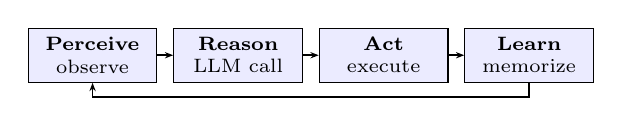
\begin{tikzpicture}[
    node distance=0.25cm,
    box/.style={rectangle, draw, fill=blue!8, text width=1.4cm, text centered, minimum height=0.5cm, font=\scriptsize},
    arrow/.style={-{Stealth[length=3pt]}, semithick},
]
    \node[box] (P) {\textbf{Perceive}\\observe};
    \node[box, right=0.2cm of P] (R) {\textbf{Reason}\\LLM call};
    \node[box, right=0.2cm of R] (A) {\textbf{Act}\\execute};
    \node[box, right=0.2cm of A] (L) {\textbf{Learn}\\memorize};
    \draw[arrow] (P) -- (R);
    \draw[arrow] (R) -- (A);
    \draw[arrow] (A) -- (L);
    \draw[arrow] (L.south) -- ++(0,-0.18) -| (P.south);
\end{tikzpicture}
\caption{The PARL decision trace loop.}
\label{fig:parl}
\end{figure}

\subsection{Trace Points and Logging}

Various trace points capture decision stages (Table~\ref{tab:trace}).

\begin{table}[ht]
\centering
\caption{Traceability capture points.}
\label{tab:trace}
\scriptsize
\begin{tabular}{@{}ll@{}}
\toprule
\textbf{Function} & \textbf{Data Captured} \\
\midrule
perceive     & Agents seen, time, location, events \\
reason       & LLM prompt, raw response, JSON action \\
execute      & Action type, target, success/failure \\
add\_memory  & Content, type, importance, agents \\
handle\_move & A* path, origin, destination, time \\
activity\_log & All actions broadcast to frontend \\
\bottomrule
\end{tabular}
\end{table}

\subsection{Cognitive State Traceability}

Each agent maintains a \textbf{CognitiveState} serving as a mental trace: \textbf{Identity Stable Set} (name, role, personality, backstory), \textbf{Action State} (status, description, duration), \textbf{Path State} (path, position, A* trace), \textbf{Conversation State} (partner, duration), and full serialization for replay.

\subsection{Memory Stream as Audit Trail}

The agent's local \textbf{memory stream} and global FAISS \textbf{MemoryStore} form an audit trail. Every observation and outcome is timestamped with an importance score (1--10).

\subsection{Anti-Repetition and Sanitization}

The engine maintains per-agent action history and a sanitization pipeline that logs hallucination corrections, target validation, and loop-breaking via console traces.

%===========================================================
\section{Simple Task Completion}
%===========================================================

\subsection{Task Lifecycle}

Agents autonomously process tasks:

\begin{enumerate}
    \item \textbf{Idle Detection:} Reasoning is triggered upon finish.
    \item \textbf{LLM Decision:} Context is sent to the LLM; JSON is parsed.
    \item \textbf{Execution:} Action dispatched (Move, Talk, Work, Rest).
    \item \textbf{Completion:} Outcome is saved, memory is formed.
\end{enumerate}

\subsection{Verified Task Completions}

Tasks verified via API during live simulation (Table~\ref{tab:tasks}).

\begin{table}[ht]
\centering
\caption{Verified task completions.}
\label{tab:tasks}
\scriptsize
\begin{tabular}{@{}llp{2.8cm}@{}}
\toprule
\textbf{Agent} & \textbf{Task} & \textbf{Outcome} \\
\midrule
Dr. Iyer   & Move: Agri Lab  & Arrived; memorized \\
Rohan      & Move: Comms     & Arrived; working \\
TARA       & Talk: Vikram    & Dialogue generated \\
Kabir      & Talk: Vikram    & Conversation done \\
Dr. Nair   & Move: Mess Hall & Arrived; reviewed \\
Dr. Reddy  & Move: Med Bay   & Arrived (teleport) \\
Cdr. Vikram& Work: logs      & Completed; stored \\
\bottomrule
\end{tabular}
\end{table}

\subsection{Conversation Trace Example}

\begin{figure}[ht]
\begin{lstlisting}[language={}]
[PARL] TARA decided: talk (Vikram)
[Conv] TARA -> Vikram (ends 06:42)
  "Good afternoon, Commander. All systems nominal."
[Conv] Ended. Memory stored.
\end{lstlisting}
\vspace{-4pt}
\caption{Sample console trace for an agent dialogue task.}
\label{fig:code_trace}
\end{figure}

%===========================================================
\section{Conclusion}
%===========================================================

The Chandrayaan-5 simulation demonstrates robust \textbf{tool integration} through 15+ REST/WebSocket endpoints and interchangeable LLM providers with FAISS semantic memory. \textbf{Agentic traceability} is achieved via PARL per-step logging, serializable cognitive states, memory audit trails, and console traces. \textbf{Task completion} is verified through autonomous decision-making, A* pathfinding, and memory-backed execution with eight concurrent agents.

% Trigger a column break right before the 1st reference to balance the last page
\IEEEtriggeratref{1}

\begin{thebibliography}{9}\itemsep=0pt\parskip=0pt
\bibitem{park2023}
J.~S.~Park \textit{et al.}, ``Generative agents: Interactive simulacra of human behavior,'' \textit{Proc. UIST}, 2023.
\bibitem{russell2020}
S.~Russell and P.~Norvig, \textit{AI: A Modern Approach}, 4th~ed., Pearson, 2020.
\end{thebibliography}

\end{document}
